\documentclass[a4paper]{article}
%% Language and font encodings
\usepackage[french]{babel}
\usepackage[utf8x]{inputenc}
\usepackage[T1]{fontenc}

%% Sets page size and margins
\usepackage[a4paper,top=3cm,bottom=2cm,left=3cm,right=3cm,marginparwidth=1.75cm]{geometry}

%% Useful packages
\usepackage{amsthm}
\usepackage{amssymb}
\usepackage{amsmath}
\usepackage{graphicx}
\usepackage{subfig}
\usepackage{wrapfig}
\usepackage[colorlinks=true, allcolors=black]{hyperref}
\usepackage{varioref}


\newcommand{\norm}[1]{\left\lVert#1\right\rVert}


\newtheorem{lem}{Lemme}
\newtheorem{theo}{Théorème}
\labelformat{theo}{le théorème~#1}
\labelformat{lem}{le lemme~#1}

\title{Rapport de TIPE}
\author{Timothée Darcet}

\begin{document}
  \maketitle

  \pagebreak

  \section{Introduction}
    Pour optimiser le processus de reconstitution d’objets en trois dimensions, nous nous étions proposé de choisir et d’implémenter en Python un tel algorithme de reconstitution, et d’en étudier l’efficacité. C’est ce que nous avons fait, en choisissant l’algorithme dit d’« enveloppe visuelle » étudié notamment par B. Baumgart [1] et A. Laurentini [2]. Il présente l’avantage d’être conceptuellement assez simple, et d’être implémentable de{} manière relativement légère.
    Nous avons donc réalisé une implémentation de cet algorithme, puis avons effectué des tests pour en étudier l’efficacité, et pouvoir analyser la pertinence des choix réalisés durant la construction de l’algorithme. Je me suis personnellement occupé de la partie de modélisation en 3D du projet, tandis que mon binôme s’est occupé du prétraitement des photographies pour les rendre exploitables. Pour s’assurer du fait que le modèle produit par l’algorithme n’est, dans des cas idéaux, pas trop éloigné de l’objet original, j’ai aussi démontré un résultat portant sur des cas simples de l’algorithme. 
  \section{Corps principal}
    \subsection{La méthode de l'enveloppe visuelle}
      L’ « enveloppe visuelle » d’un objet A est l’objet maximal qui donne la même silhouette que A quand on l’observe depuis un ensemble de points de vue donné. Ainsi, l’enveloppe visuelle de A depuis un point de vue unique est un cône dont le sommet est placé sur ce point de vue, et qui a la forme de la silhouette de A depuis ce point de vue (fig. 1).

      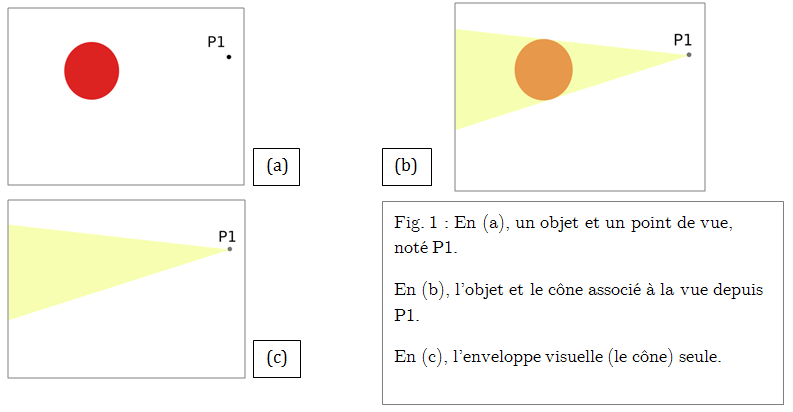
\includegraphics[width=\textwidth]{ScreenSchema1}      

      Pour obtenir l’enveloppe visuelle d’un objet depuis plusieurs points de vue, on peut alors simplement considérer l’intersection des enveloppes visuelles obtenues depuis chacun des points de vue. Un exemple (en deux dimensions, pour simplifier) est donné en fig. 2.

      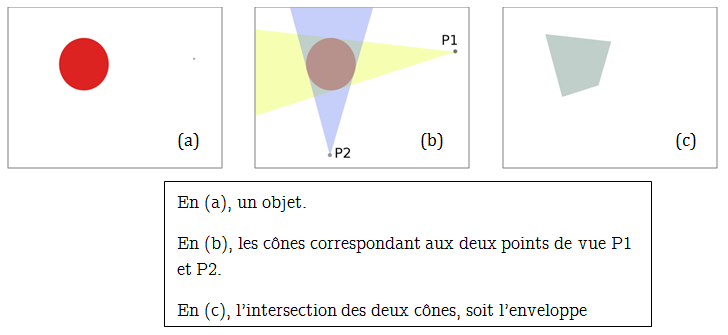
\includegraphics[width=\textwidth]{ScreenSchema2}

      En multipliant les points de vue, l’enveloppe visuelle se rapproche de l’objet original. On peut donc utiliser cette méthode pour reconstituer le modèle 3D d’un objet, simplement à partir de photographies. Se dégagent alors deux étapes majeures pour cette reconstitution :

      \begin{itemize}
        \item Le traitement de la photographie, pour dégager la silhouette de l’objet :\\
        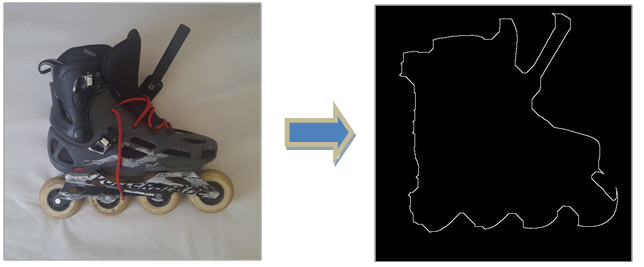
\includegraphics[width=\linewidth]{ContourDetect}
        \item La reconstitution à proprement parler, qui consiste à créer les cônes correspondant aux silhouettes, puis à en calculer l’intersection.
      \end{itemize}


      Ma contribution personnelle fut la démonstration d’un résultat sur l’enveloppe visuelle, qui permet d’établir un lien entre un objet et son enveloppe visuelle, et la construction d’un système de représentation en machine d’objets en 3D, ainsi que de tous les algorithmes l’accompagnant, en particulier les algorithmes d’intersection, de constructions de cônes, et de simulation de la prise d’une photographie. Cette construction fut réalisée en langage python.

    \subsection{Une formalisation mathématique}
      Formellement, une photographie est une projection plane relative à un foyer. Ainsi, si on munit $\mathbb{R}^{3}$ de son produit scalaire canonique $(\cdot|\cdot)$, on peut, pour un foyer $f \in \mathbb{R}^3$ et un point du plan image $p$, poser
      
      \[
      \begin{array}{ccrcl}
        p_{f, p} & : & \mathbb{R}^{3}\setminus\{x \in \mathbb{R}^3 | (x - f | p - f) = 0\} & \to     & \mathbb{R}^{3}\\
          &   & x              & \mapsto & f + \frac{\norm{p - f}^2}{(x - f | p - f)} \cdot (x - f)\\
      \end{array}
      \]

      On remarque que pour tout $x \in \mathbb{R}^3$, il existe $\lambda \in \mathbb{R}$ tel que $p(x) - f = \lambda (x - f)$, donc $f$, $x$ et $p(x)$ sont alignés.\\
      De plus pour tout $x$ pour lequel $p(x)$ est défini, $(p(x) - f | p - f) = (p - f | p - f)$ donc $p(x)$ est bien dans le plan de vecteur normal $p - f$ qui passe par p.\\
      Ainsi p correspond bien à une photographie.\\
      \\
      On peut alors poser, pour une partie $A$ de $\mathbb{R}^3$ et un ensemble $V$ de couples $(f, p) \in \mathbb{R}^3$ où f représente un foyer et p un point d'un plan image, l'enveloppe visuelle de $A$ relative à l'ensemble de points de vues $V$:
      
      \[ev(V, A) = \bigcap_{(f, p) \in V}\{f + \lambda \cdot (y - f), \lambda \in \mathbb{R}+, y \in p_{f, p}(A)\}\]

      (On notera que ceci correspond au cas théorique ou le plan de projection est situé entre le foyer et l'objet, alors qu'une photographie réelle utilise un plan de projection tel que le foyer soit entre ce plan et l'objet. Cela ne perturbera pas les résultats.)\\
      \\
      L'enveloppe visuelle étant formalisée, on peut montrer des résultats dessus.\\
      Premièrement, si un objet est bien entièrement du "bon" coté des plans images choisis, c'est-à-dire que chaque plan image est entre l'objet et le foyer correspondant, alors son enveloppe visuelle ne dépend pas des plans images choisis, et elle peut s'exprimer plus simplement :

      \[
      ev(V, A) = \bigcap_{(f, p) \in V} \{f + \lambda \cdot (x - f), \, \lambda \in \mathbb{R}+, x \in A\}
      \]

      La démonstration pourra être retrouvée \hyperref[AnnexeA]{annexe A}.

      Un corollaire est que pour un objet qui satisfait ces hypothèses, l'objet sera toujours inclus dans son enveloppe visuelle relative à un ensemble de points de vues quelconques.

      Un autre résultat que l'on peut alors montrer est que, étant donné une sphère $S$ qui contient l'objet $A$, l'enveloppe visuelle de $A$ relative aux points de vues situés sur $S$ est  incluse dans l'enveloppe convexe de $A$. La démonstration de ce résultat est fournie en \hyperref[AnnexeB]{annexe B}.

    \subsection{L'implémentation en machine}
      Deux principaux types de stockage en mémoire des objets 3D existent :
      \begin{itemize}
        \item L'approximation par des polyèdres.
        \item La modélisation par des "voxels", c'est-à-dire des "pixels de volume". L'espace est alors représenté par une grille finie, où chaque case peut prendre plusieurs états, par exemple "remplie" ou "vide".
      \end{itemize}
      \begin{figure}[h]%
          \centering
          \subfloat[Des voxels]{{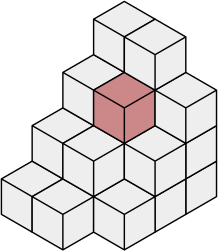
\includegraphics[width=0.3\linewidth]{Voxels} }}%
          \qquad
          \subfloat[Un polyèdre]{{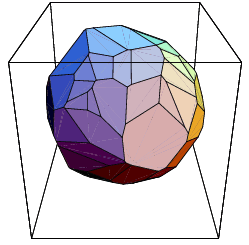
\includegraphics[width=0.3\linewidth]{Polyhedron} }}%
          \caption{Une comparaison entre polyèdre et voxels}%
          \label{fig1}%
      \end{figure}

      
      La modélisation précise que nous avons choisi est la modélisation par "polyèdre aux arêtes ailées" ("winged edge polyhedron") introduite par B. Baumgart. Elle utilise quatre types d'objets distincts:
      \begin{itemize}
        \item Les objets polyèdres, qui stockent une liste de faces, une liste de sommets et une liste d'arêtes
        \item Les sommets, qui stockent leurs trois coordonnées ainsi qu'un lien vers une de leurs arête
        \item Les faces, qui stockent un lien vers une arête adjacente
        \item Les arêtes, qui stockent huits liens, nommés selon la figure \ref{fig1} :
        \begin{itemize}
          \item \texttt{PVT} et \texttt{NVT} pointent vers les sommets aux extrémités de l'arête
          \item \texttt{NFACE} et \texttt{PFACE} pointent vers les faces adjacentes à l'arête
          \item \texttt{PCW}, \texttt{NCW}, \texttt{PCCW} et \texttt{NCCW} pointent vers les quatre "ailes" (qui donnent ce nom à la modélisation): ce sont les arêtes qui ont un sommet et une face en commun avec l'arête considérée.
        \end{itemize}
      \end{itemize}

      \begin{figure}
        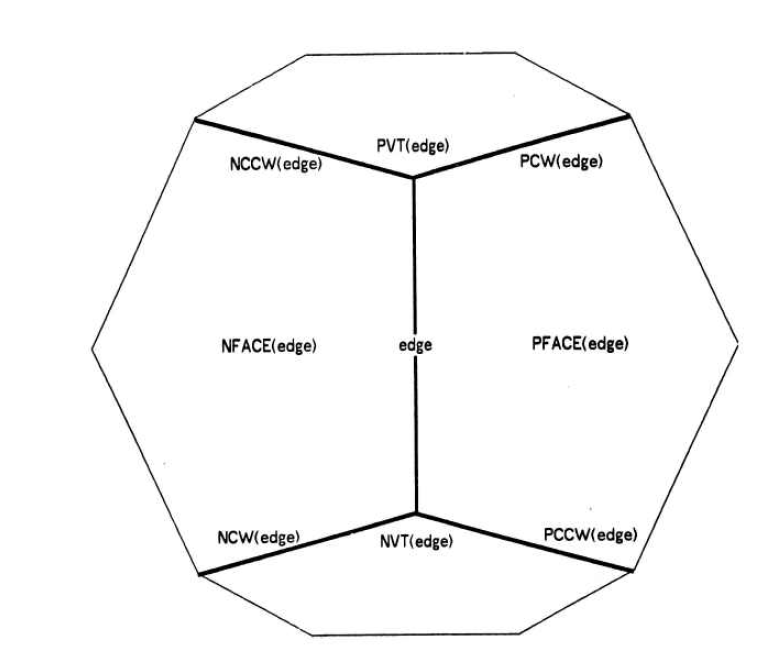
\includegraphics[width=0.5\linewidth]{WEP}
        \centering
        \caption{Les liens que stockent une arête dans le modèle du "winged edge polyhedron"}
        \label{fig1}
      \end{figure}

      Ainsi un polyèdre cohérent peut être défini. On remarquera que seuls les sommets possèdent des informations sur les positions des éléments dans l'espace, tandis que les arêtes stockent toutes les informations de structure (quels éléments sont liés auxquels). Les faces, quant à elles, donnent des indication sur le caractère visuel du polyèdre: ce sont elles qui vont bloquer ou non la lumière, et ainsi elles seront utiles pour simuler une vue de l'objet.\\
      Cette dissociation des informations stockées en mémoire est intéressante : ainsi, on peut facilement déformer un polyèdre tout en gardant sa topologie, en appliquant une fonction vectorielle aux seules coordonnées des sommets.\\
      \\
      \subsection{Les tests effectués}
      A partir de cette modélisation, j’ai réalisé des tests sur l’algorithme d’intersection pour obtenir des informations sur le temps d’exécution de cet algorithme pour divers complexités de polyèdres initiaux. Nous avons préféré une analyse du temps d’exécution pratique plutôt qu’une étude de la complexité théorique. En effet, si cette dernière donne des bonnes informations asymptotiques, elle ne donne aucun contrôle sur la vitesse de convergence, et un algorithme en O(n²) pourra être en pratique beaucoup plus rapide à exécuter qu’un autre qui est en O(n), simplement parce que les n considérés ne deviennent jamais très grands. De plus, une information sur le temps d’exécution, en secondes, est bien plus facilement interprétable qu’une information de complexité. Ainsi, des tests simples sur le programme que j’ai réalisé montrent qu’une intersection simple, avec deux polyèdre ayant de l’ordre de la dizaine de sommets, prend en moyenne 0,15s sur un ordinateur portable, le processeur y étant cadencé à 2 GHz. Ceci, bien sûr, n’est que le temps d’exécution sur une machine particulière, et en utilisant des machines plus puissantes, ce temps pourrait être considérablement réduit. Mais il faut reprendre les objectifs que nous nous étions fixés : nous cherchions un algorithme efficace, qui renvoie des résultats les plus fidèles possibles tout ayant un temps d’exécution le plus court possible. Ici, les résultats obtenus signifient que pour pouvoir reconstituer un modèle 3D avec une précision acceptable, en un temps raisonnable (c’est-à-dire réaliser de l’ordre de 10 à 100 intersections de polyèdres qui possèdent de l’ordre de 1000 sommets), il faudrait une machine très puissante.

  \appendix
  \section{Annexe}\label{AnnexeA}
    Soit une partie $A$ de $\mathbb{R}^3$ et un ensemble $V$ de couples $(f, p) \in \mathbb{R}^3$ où f représente un foyer et p un point d'un plan image. On suppose que pour tout élément $x$ de $A$, pour tout $(f, p) \in V$,  
    \[(x - f | p - f) > 0\]
    Ce qui signifie que le plan normal à $p - f$ passant par $p$ (le plan image) est entre $f$ et $x$.
    Soit $(f, p) \in V$
    \begin{align*}
      \{f + \lambda \cdot (y - f), \lambda \in \mathbb{R}+, y \in p_{f, p}(A)\}
      &= \{f + \lambda \cdot \frac{\norm{p - f}^2}{(x - f | p - f)} \cdot (x - f), \lambda \in \mathbb{R}+, y \in p_{f, p}(A)\}\\
      &= \{f + \mu \cdot (x - f), \mu \in \mathbb{R}+, y \in p_{f, p}(A)\}\\
    \end{align*}
    On a donc bien que
    \[
      ev(V, A) = \bigcap_{(f, p) \in V} \{f + \lambda \cdot (x - f), \, \lambda \in \mathbb{R}+, x \in A\}
    \]
  \section{Annexe}\label{AnnexeB}
    Nous nous plaçons dans le $\mathbb{R}$-espace vectoriel $E = \mathbb{R}^{3}$, muni de sa structure d'espace euclidien canonique, pour laquelle le produit scalaire sera noté $(\cdot|\cdot)$


    Pour tout $x\in E$, on définit le projecteur de foyer $x$ comme :

    \[\begin{array}{ccccl}
    p_{x} & : & E\setminus\{x\} & \to & S(x, 1) \\
     & & y & \mapsto & x  + \frac{1}{\norm{y - x}} \cdot (y - x) \\
    \end{array}\]

    (On notera $S(x, r)$, $B_{o}(x, r)$ et $B_{f}(x, r)$ respectivement la sphère, la boule ouverte et la boule fermée de centre $x$ et de rayon $r$)


    On définit la silhouette d'une  partie $A$ de $E$ vue depuis un point $x$ comme son image directe par $p_{x}$.

    \textit{Note : Cela ne correspond pas exactement à une photographie, qui elle est une projection sur un plan. Toutefois, on admettra que si un objet est entièrement du coté du plan focal opposé au foyer (ce qui est toujours vérifié pour une photographie), le "cône" reconstruit à partir de sa photographie est le même que celui reconstruit à partir de la projection sphérique, et que donc la définition de l'enveloppe visuelle que l'on va donner ici correspond donc bien à la définition "naturelle".}

    On définit ensuite le cône de sommet $x$ et de silhouette $A \subset S(x, 1)$ comme suit:

    \[C(x,A) = \{\,x + t\cdot{}(y - x), y\in{}A, t\in\mathbb{R}+\,\}\]

    On peut alors définir l'enveloppe visuelle d'une partie $A$ de $E$ selon un ensemble de points de vues $V$ :

    \[ev(V, A) = \bigcap_{x\in{}V}C(x,p_{x}(A))\]

    On notera aussi $conv(A)$ l'enveloppe convexe de $a$, et on admettra que :

    \[conv(A) = \{\,\sum_{i=1}^{n} \lambda_{i} x_{i}| n\in{}\mathbb{N}^{*}, (x_{i})_{1\leqslant i \leqslant n} \in E^{n}, \, (\lambda_{i})_{1\leqslant i \leqslant n} \in [0, 1]^{n}\text{ t.q. } \sum_{i=1}^{n} \lambda_{i} = 1\}\]

    J'ai montré dans un premier temps \ref{lem1}:\\*
    \begin{lem}\label{lem1}

    \textbf{Si} $A$ est un fermé de $E$, et il existe $b \in E$ et $M \in \mathbb{R}$ tels que $A \subset B_{o}(b, M)$,

    \[\textbf{Alors } ev(S(b,M), A) \subset B_{o}(b, M)\]

    \end{lem}

    \begin{proof}

    On supposera, quitte à faire effectuer une translation à $A$, que $b = 0$

    Supposons qu'il existe $x \in ev(S(0,M), A)$ tel que $\norm{x} \geqslant M$

    \begin{itemize}
    \item Si $\norm{x} > M$ 

    On considère $\beta$ un vecteur orthogonal à $x$ de norme $1$ ($\beta$ existe car $E$ est un espace euclidien de dimension $3$)

    On pose $y = \frac{M^{2}}{\norm{x}^{2}} \cdot x + M \sqrt{1 - \frac{M^{2}}{\norm{x}^{2}}} \cdot \beta$

    On remarque que 

    \begin{align*}
    \norm{y}^{2} &= \frac{M^{4}}{\norm{x}^{2}} + M^{2} (1 -\frac{M^{2}}{\norm{x}^{2}}) \\
                 &= M^{2}\\
    \end{align*}

    Donc que $y \in S(0, M)$

    Et que

    \begin{align*}
    (y|x - y) &= (y|x) - \norm{y}^{2}\\
              &= M^{2} - M^{2}\\
              &= 0\\
    \end{align*}

    Or $y \in S(0, M)$ donc $x \in C(y, p_{y}(A))$, donc il existe $u\in p_{y}(A)$ et $t\in \mathbb{R}+$ tels que $x = y + t \cdot (u - y)$.

    Comme $\norm{x} > M$, $t\neq 0$

    Donc $u - y = \frac{1}{t} \cdot (x - y)$, et donc $(u - y|y) = 0$

    De plus $u \in p_{y}(A)$ donc il existe $v \in A$ tel que $u = y + \frac{1}{\norm{v -  y}} \cdot (v - y)$

    Donc $v = y + \norm{v - y} \cdot (u - y))$

    Comme $(u - y|y) = 0$,

    \begin{align*}
    \norm{v}^{2} &= \norm{y}^{2} + \norm{v - y}^{2} \cdot \norm{u - y}^{2} \\
                 &\geqslant M^{2} \\
    \end{align*}


    Or, par hypothèse, $v \in A$ implique $\norm{v} < M$

    On a une contradiction.

    \bigskip

    \item Si  $\norm{x} = M$

    $A$ est fermé et borné car inclus dans $B_{o}(0, M)$, donc $A$ est compact (On a $dim(E) = 3$).

    Et comme $u \mapsto \norm{u}$ est continue, elle admet un maximum $n_{m}$ sur $A$. Il existe donc $x_{0} \in A$ tel que $\norm{x_{0}} = n_{m}$

    $x_{0} \in B_{o}(0, M)$ donc $n_{m} < M$

    Soit $y$ un vecteur de $S(0, M)$ tel que $\norm{y - x} < \frac{M - n_{m}}{2}$ et $y \neq x$

    $y \in S(0, M)$ donc $x \in C(y, p_{y}(A))$

    Donc il existe $v \in A$ et $t \in \mathbb{R}+$ tel que $x = y + \frac{t}{\norm{v - y}} \cdot (v - y)$

    $x \neq y$ donc $t \neq 0$ et $v = y + \frac{\norm{v - y}}{t} \cdot (x - y)$

    On note 
    \[\begin{array}{ccccl}
    f & : & \mathbb{R} & \to & \mathbb{R} \\
     & & \lambda & \mapsto & \norm{y}^{2} + \lambda^{2} \cdot \norm{x - y}^{2} + 2 \lambda (y|x - y)\\
    \end{array}\]

    (On a alors $f(\lambda) = \norm{y + \lambda \cdot (x - y)}^{2}$, et donc $\norm{v}^{2} = f(\frac{\norm{v - y}}{t})$)

    Or $f'(\lambda) = 2 \lambda \norm{x - y}^{2} + 2(y|x - y)$

    Donc $f(\lambda)$ atteint un minimum en
    \[\lambda = \frac{(y|y - x)}{\norm{x - y}^2} = \frac{\norm{y}^{2} - (y|x)}{\norm{x}^{2} + \norm{y}^{2} - 2 (x|y)} = \frac{1}{2}\]
    (Car $\norm{x} = \norm{y}$)

    \medskip

    Ainsi 
    \begin{align*}
    \norm{v}^{2} &= f(\frac{\norm{v - y}}{t}) \\
                 &\geqslant f(\frac{1}{2}) \\
                 &\geqslant \norm{y + \frac{1}{2} (x - y)}^{2} \\
                 &\geqslant (\norm{y} - \frac{1}{2} \norm{x - y})^{2} \\
    \end{align*}

    Donc $\norm{v} \geqslant \norm{y} - \frac{1}{2} \norm{x - y}$

    Or, par construction de y, $\norm{y - x} < \frac{M - n_{m}}{2}$

    Donc $\norm{v} > n_{m}$

    Or $v \in A$  donc $\norm{v} \leqslant n_{m}$
    On a encore une contradiction.
    \end{itemize}

    \medskip

    Dans les deux cas on a une contradiction.
    Donc $\norm{x} < M$
    \end{proof}

    \bigskip

    J'ai ensuite montré \ref{th1} :\\*
    \begin{theo}\label{th1}

    L'enveloppe visuelle d'un fermé $A$ de $E$ vu depuis une sphère englobant A est incluse dans l'enveloppe convexe de $A$.

    En d'autres termes, 
    \begin{gather*}
    \forall A \subset E \text{ t.q. $A$ fermé et borné, } \forall (b, M) \in E \times \mathbb{R} \text{ t.q. } A \subset B_{o}(b, M), \\
    \text{On a } ev(S(b, M), A) \subset conv(A)
    \end{gather*}
    \end{theo}


    \begin{proof}
    Soit $A$ un fermé de $E$

    On considérera $A$ non vide (Si $A$ est vide, $ev(S(b, M), A) = conv(A) = A = \varnothing$)

    Soit $a \in ev(S(b, M), A)$

    Quitte à effectuer une translation sur $A$ et $b$, on va considérer que $a = 0_{E}$.

    \begin{itemize}
    \item Si $0 \in A$, immédiatement $0 \in conv(A)$
    \bigskip
    \item Si $0 \notin A$, on a que $\forall x \in S(b, M), 0 \in C(x, p_{x}(A))$

    Donc \[\exists t \in \mathbb{R}+, \exists y\in p_{x}(A) \text{ t.q. } 0 = x + t \cdot (y - x)\]

    Or $y \in p_{x}(A)$ donc il existe $z$ dans $A$ tel que $p_{x}(z) = y$, soit

    \[y - x = \frac{1}{\norm{z - x}} \cdot (z - x)\]


    Soit $x_{0} \in S(0, 1)$

    On note alors
    \[\begin{array}{ccccl}
    d& : & \mathbb{R} & \to & E \\
     & & t & \mapsto & t \cdot x_{0} \\
    \end{array}\]

    $d(\mathbb{R})$ est la droite passant par $x_{0}$  et par $0$.

    De plus $A \subset B_{o}(b, M)$ et $0 \in ev(S(b, M), A)$ donc, selon \ref{lem1}, $\norm{0 - b} < M$

    Ainsi $\norm{d(0) - b} < M$, et comme $\lim_{t \to +\infty}\norm{d(t)} = +\infty$ et $t \mapsto \norm{d(t) - b}$ est une application continue, selon le théorème des valeurs intermédiaires,

    \[\exists t_{1} \in \mathbb{R}\setminus\{0\} \text{ tel que } \norm{d(t_{1})} = M\]

    On note $x_{1} = d(t_{1})$

    Comme $0 \in C(x_{1}, p_{x_{1}}(A))$, il existe $v \in A$ et $\lambda \in \mathbb{R}+$ tels que \[0 = x_{1} + \lambda (v - x_{1})\]

    De plus $\lambda \neq 0$, donc \[v = \frac{\lambda - 1}{\lambda} \cdot x_{1} = t_{1} \cdot (1 - \frac{1}{\lambda}) x_{0}\]

    Ainsi, selon le signe de $t_{1} \cdot (1 - \frac{1}{\lambda})$, on aura $p_{0}(v) = x_{0}$ ou $p_{0}(v) = - x_{0}$

    Cela est vrai pour tout $x_{0}$ dans $S(0, 1)$ donc, en notant $P = p_{0}(A)$ et $P' = \{-a, a \in P \}$, $P \cup P' = S(0, 1)$

    \bigskip

    On cherche alors à montrer que $ P \cap P' \neq \varnothing$

    Comme $A$ est fermé et borné en dimension finie, $A$ est compact, et comme $p_{0}$ est continue, $P = p_{0}(A)$ est compact aussi.

    Et comme $a \mapsto -a$ est continue, $P'$ est compact aussi.

    Soit alors $u \in P$ et $v$ un vecteur orthogonal à $u$ de norme $1$

    On note 
    \[\begin{array}{ccccl}
    \gamma & : & [0, 1] & \to     & S(0, 1) \\
           &   & t      & \mapsto & cos(t\pi) \cdot u + sin(t\pi) \cdot v \\
    \end{array}\]

    $\gamma$ est continue, donc $\gamma^{-1}(P)$ et $\gamma^{-1}(P')$ sont fermés.

    $\gamma(0) = u \in P$ donc $\gamma^{-1}(P) \neq \varnothing$ et on peut donc considérer $t = \sup \gamma^{-1}(P) = \max \gamma^{-1}(P)$ (Car $\gamma^{-1}(P)$ est fermé)

    \begin{itemize}
    \item Si $t = 1$, $-u \in P$, et comme on a aussi $u \in P$, $u \in P \cap P'$
    \medskip
    \item Si $t < 1$, il existe $n_{0} \in \mathbb{N}$ tel que $\forall n \geqslant n_{0}, t + \frac{1}{n} \leqslant 1$
    Alors $(\gamma(t + \frac{1}{n}))_{n \geqslant n_{0}}$ est une suite d'éléments qui ne sont pas dans $P$, et donc qui sont dans $P'$ (car ils sont dans $S(0, 1)$)


    Comme $\gamma$ est continue, elle converge vers $\gamma(t)$, et comme $P'$ est fermé, on a donc $\gamma(t) \in P'$

    Donc $\gamma(t) \in P \cap P'$
    \end{itemize}

    On a donc que $P \cap P'$ est non vide

    \bigskip

    Soit $q$ un élément de $P \cap P'$

    On a $q \in p_{0}(A)$ donc il existe $\mu \in \mathbb{R}+$ tel que $\mu q \in A$

    De même $-q \in p_{0}(A)$ donc il existe $\nu \in \mathbb{R}+$ tel que - $\nu q \in A$

    $0_{E} \notin A$ donc $\mu \neq 0$ et $\nu \neq 0$

    on note $\alpha = \frac{\frac{1}{\mu}}{\frac{1}{\mu} + \frac{1}{\nu}}$ (on a $\alpha \in [0, 1]$)

    Ainsi $0_{E} = \alpha \cdot \mu q + (1 - \alpha) \cdot (- \nu  q)$

    Donc $0_{E} \in \{c \cdot u + (1 - c) \cdot v, c \in [0, 1], (u, v) \in A^{2} \}$


    Et donc $0_{E} \in conv(A)$
    \end{itemize}
    \end{proof}
\end{document}